We will in this chapter discuss radially sheared poloidal flows with $m_\theta = 0$ in short.
Such flows have gained a lot attention in the recent years due to its ability to suppress the turbulence transport through decorrelation of eddies, and is associated with transport barriers and the high confinement mode in tokamaks \cite{Terry2000,Diamond2005a,Viezzer2012Phd}.
In plasma physics, one sometimes distinguish between a time fluctuating "zonal flow"%
\footnote{The term "zonal flow" is used in meteorology to describe atmospheric and oceanic circulation along latitudinal lines, such as those observed in Jupiter \cite{Limaye1986}.}%
, and a time stationary mean background poloidal flow.

The zonal flow can be initiated through a parametric decay of drift-waves to an $m_\theta=0$ wave together with a modulation instability of the same waves \cite{Diamond2005a}.
Once initiated, it sets up a predator-prey relationship between the turbulence and the zonal flow.
The turbulence drives a zonal flow which suppresses the turbulence.
When the turbulence is suppressed the zonal flow is not fed, so it dies out.
This means that the turbulence grows up, and the story repeats itself.

The mechanisms behind the time stationary flow can be found by investigating the force balance in the ion momentum equation%
\footnote{The ions are investigated rather than the electrons as the momentum is mainly carried by the ions due to the mass difference.}%
%
.
From such a consideration, one find that a poloidal background flow can be created through a radial electric field generated by a strong radial ion pressure gradient, by a radial gradient in the Reynold stresses
\footnote{Stresses on the mean flow generated by turbulence.
See \cite{Kundu2010book} for details.}%
and plasma rotation \cite{Terry2000}.
Notice that a poloidal mean flow may also develop if the radial boundary conditions causes gradients in $\phi$.
Reference \cite{Tynan2006a} suggest that inverse cascading (through the Reynolds stresses) of the turbulent energy is a generation mechanism of their observed steady poloidal mean flow in a cylindrical device like the one we have simulated here.
The shear is visible both through the radial profile of the velocity, and through a suppressed turbulence outside the shear visible from the radial power spectrum density.

It is therefore interesting to see whether such a poloidal mean flow is observed in our simulations.
As we do not have accounted for the ion pressure in our model, a radial pressure gradient is ruled out as a candidate for any possibly observed poloidal flow.
We can also rule out plasma rotation as we are looking at a linear device.
Remaining candidates for poloidal flows are therefore Reynold stresses and the zonal flows and flows arising from the boundaries.
The acceleration in poloidal flow can be found from the material time derivate of the vorticity, and yields \cite{Diamond1991}
%
\begin{align*}
    \partial_t \expt{\ve{u}_{E\times B,\theta}}_t = \expt{\partial_\rho\L(\wt{\ve{u}}_{E\times B,\rho}\wt{\ve{u}}_{E\times B,\theta}\R)}_t.
\end{align*}
%

%
\begin{figure}[htbp]
    \centering
    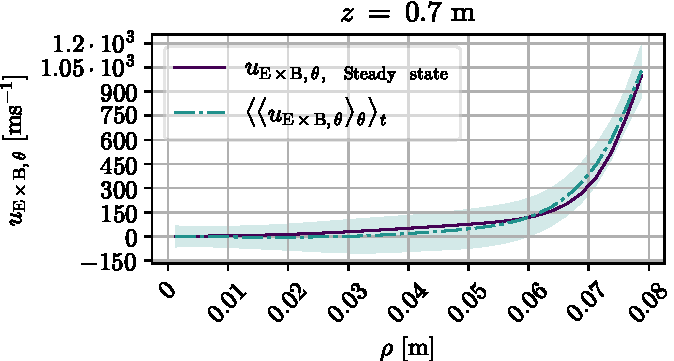
\includegraphics{fig/results/poloidalFlow/poloidalFlow01}
    \caption{Poloidal velocity in the system for $B=0.01\T$.
        The solid line represents the steady state, the dashed line the temporal and poloidal mean in the saturated turbulence phase.
        The shaded area represents the standard deviation found in the turbulent phase.}
    \label{fig:poloidalFlow0008}
\end{figure}
%
\Cref{fig:poloidalFlow0008} shows the radial poloidal velocity profile from our simulations.
We can observe a strong poloidal shear at the edge of the plasma in the steady state.
This is attributed to the strong potential gradient which is a result of our boundary conditions as mentioned in \cref{chap:ss}.
Although we found in \cref{chap:charTurb} the turbulence modifies the profiles, we can observe that the mean of the turbulence phase do not deviate much from the steady state solution (less than $10\%$ at max).
In other words the fluctuations in the poloidal velocity oscillates around the mean.
Despite having poloidal velocity fluctuation levels in the orders of $10\%$, no large suppression of the density fluctuations observed in \cref{fig:PSD2D}.
The spectral broadening is in qualitative accordance with what was found in \cite{Tynan2006a}, albeit a broader spectra was found in the reference.
However, the shear and the resulting suppression of turbulence is not found in this work.
This suggest that either a broader turbulence spectra is needed for the poloidal shear velocity to occur, that the ion dynamics which we have ignored is important, or it comes as a result of the differences between the numerical and experimental set-up.
%
\begin{figure}[htbp]
    \centering
    \begin{subfigure}[h]{1\textwidth}
        \centering
        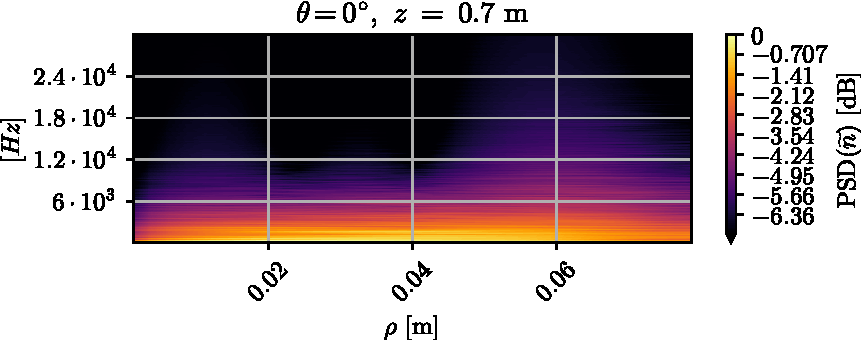
\includegraphics{fig/results/poloidalFlow/PSD2D006}
        \label{fig:PSD2D006}
        \caption{$B=0.06\T$}
    \end{subfigure}%
    \\
    \begin{subfigure}[h]{1\textwidth}
        \centering
        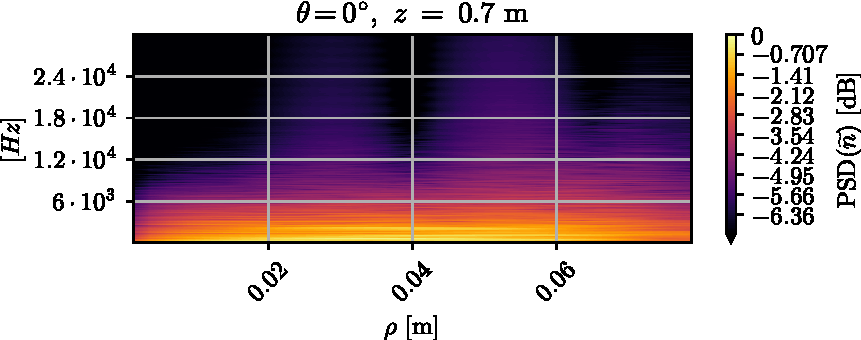
\includegraphics{fig/results/poloidalFlow/PSD2D008}
        \label{fig:PSD2D008}
        \caption{$B=0.08\T$}
    \end{subfigure}
    \\
    \begin{subfigure}[h]{1\textwidth}
        \centering
        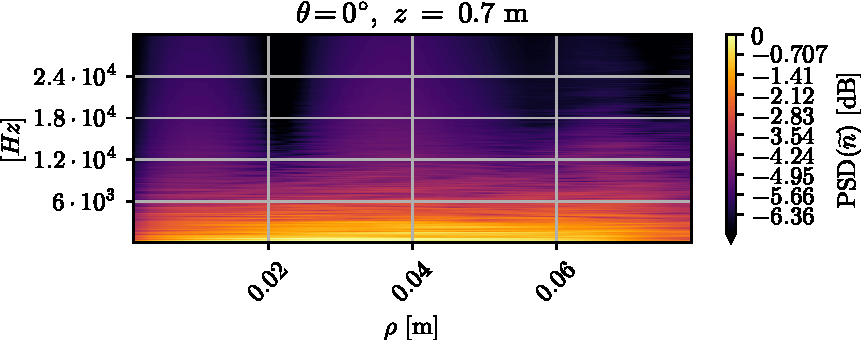
\includegraphics{fig/results/poloidalFlow/PSD2D01}
        \label{fig:PSD2D008B}
        \caption{$B=0.01\T$}
    \end{subfigure}
    \caption{Radial dependency on the power spectral density.}
    \label{fig:PSD2D}
\end{figure}
%
